%TODO parler de formation planétaire (en citant des papiers, sans rentrer dans les détails. notamment pollack, alibert)

%TODO une des grandes questions c'est  : comment on forme des noyaux de jupiter et Kepler 11?

%TODO voir l'intro de franckH et en particulier la partie sur laplace et descartes?

Oscillant en fonction de l'humeur de l'époque le débat de la vie ailleurs et de l'existence d'autres planètes a animé la communauté scientifique depuis l'antiquité. Souvent influencé par les convictions religieuses et les modèles du système solaire en vigueur, il était parfois même dangereux d'émettre l'hypothèse que d'autres planètes ou d'autres formes de vies puissent exister, l'idée de la pluralité des civilisations étant indissociable de la question de la pluralité des mondes physiques. %TODO continuer la partie histoire des sciences et pluralité des mondes.

Ces questions que l'on pouvait considérer comme philosophiques ou métaphysiques ont changé de registre depuis la découverte, il y a une vingtaine d'années de la première exoplanète\footnote{Planète orbitant autour d'une étoile autre que notre Soleil.} \citep{1992Natur.355..145W}.

Bien que cette dernière fut découverte en 1992, c'est véritablement en 1995 avec \object{51 Peg b} \citep{mayor1995jupiter} que la chasse aux exoplanètes a véritablement commencé. Depuis, multipliant les campagnes d'observations, les missions dédiées et les techniques de détection, on arrive, 20 ans après la première découverte à un catalogue d'exoplanètes toujours plus fourni, montrant une population extrêmement riche et variée. Le nombre variant continuellement, il n'y a pas de sens à donner un chiffre sans la date associée mais au jour du 20 février 2013, on compte pas moins de 861 planètes confirmées. 

Avant toute chose, il est important de noter le nombre. Non pas le nombre exact mais plutôt les conséquences qu'implique une liste de plusieurs centaines de planètes : Ce ne sont pas des objets rares ! Si auparavant on pouvait encore en douter, il ne fait aujourd'hui plus aucun doute que les planètes sont des objets communs. C'est d'autant plus flagrant quand on note que la grande majorité des exoplanètes détectées l'ont été autour d'étoiles à moins de 400 pc du Soleil comme illustré dans \reffig{fig:milky_way_exoplanet}. 

\begin{figure}[htb]
\centering
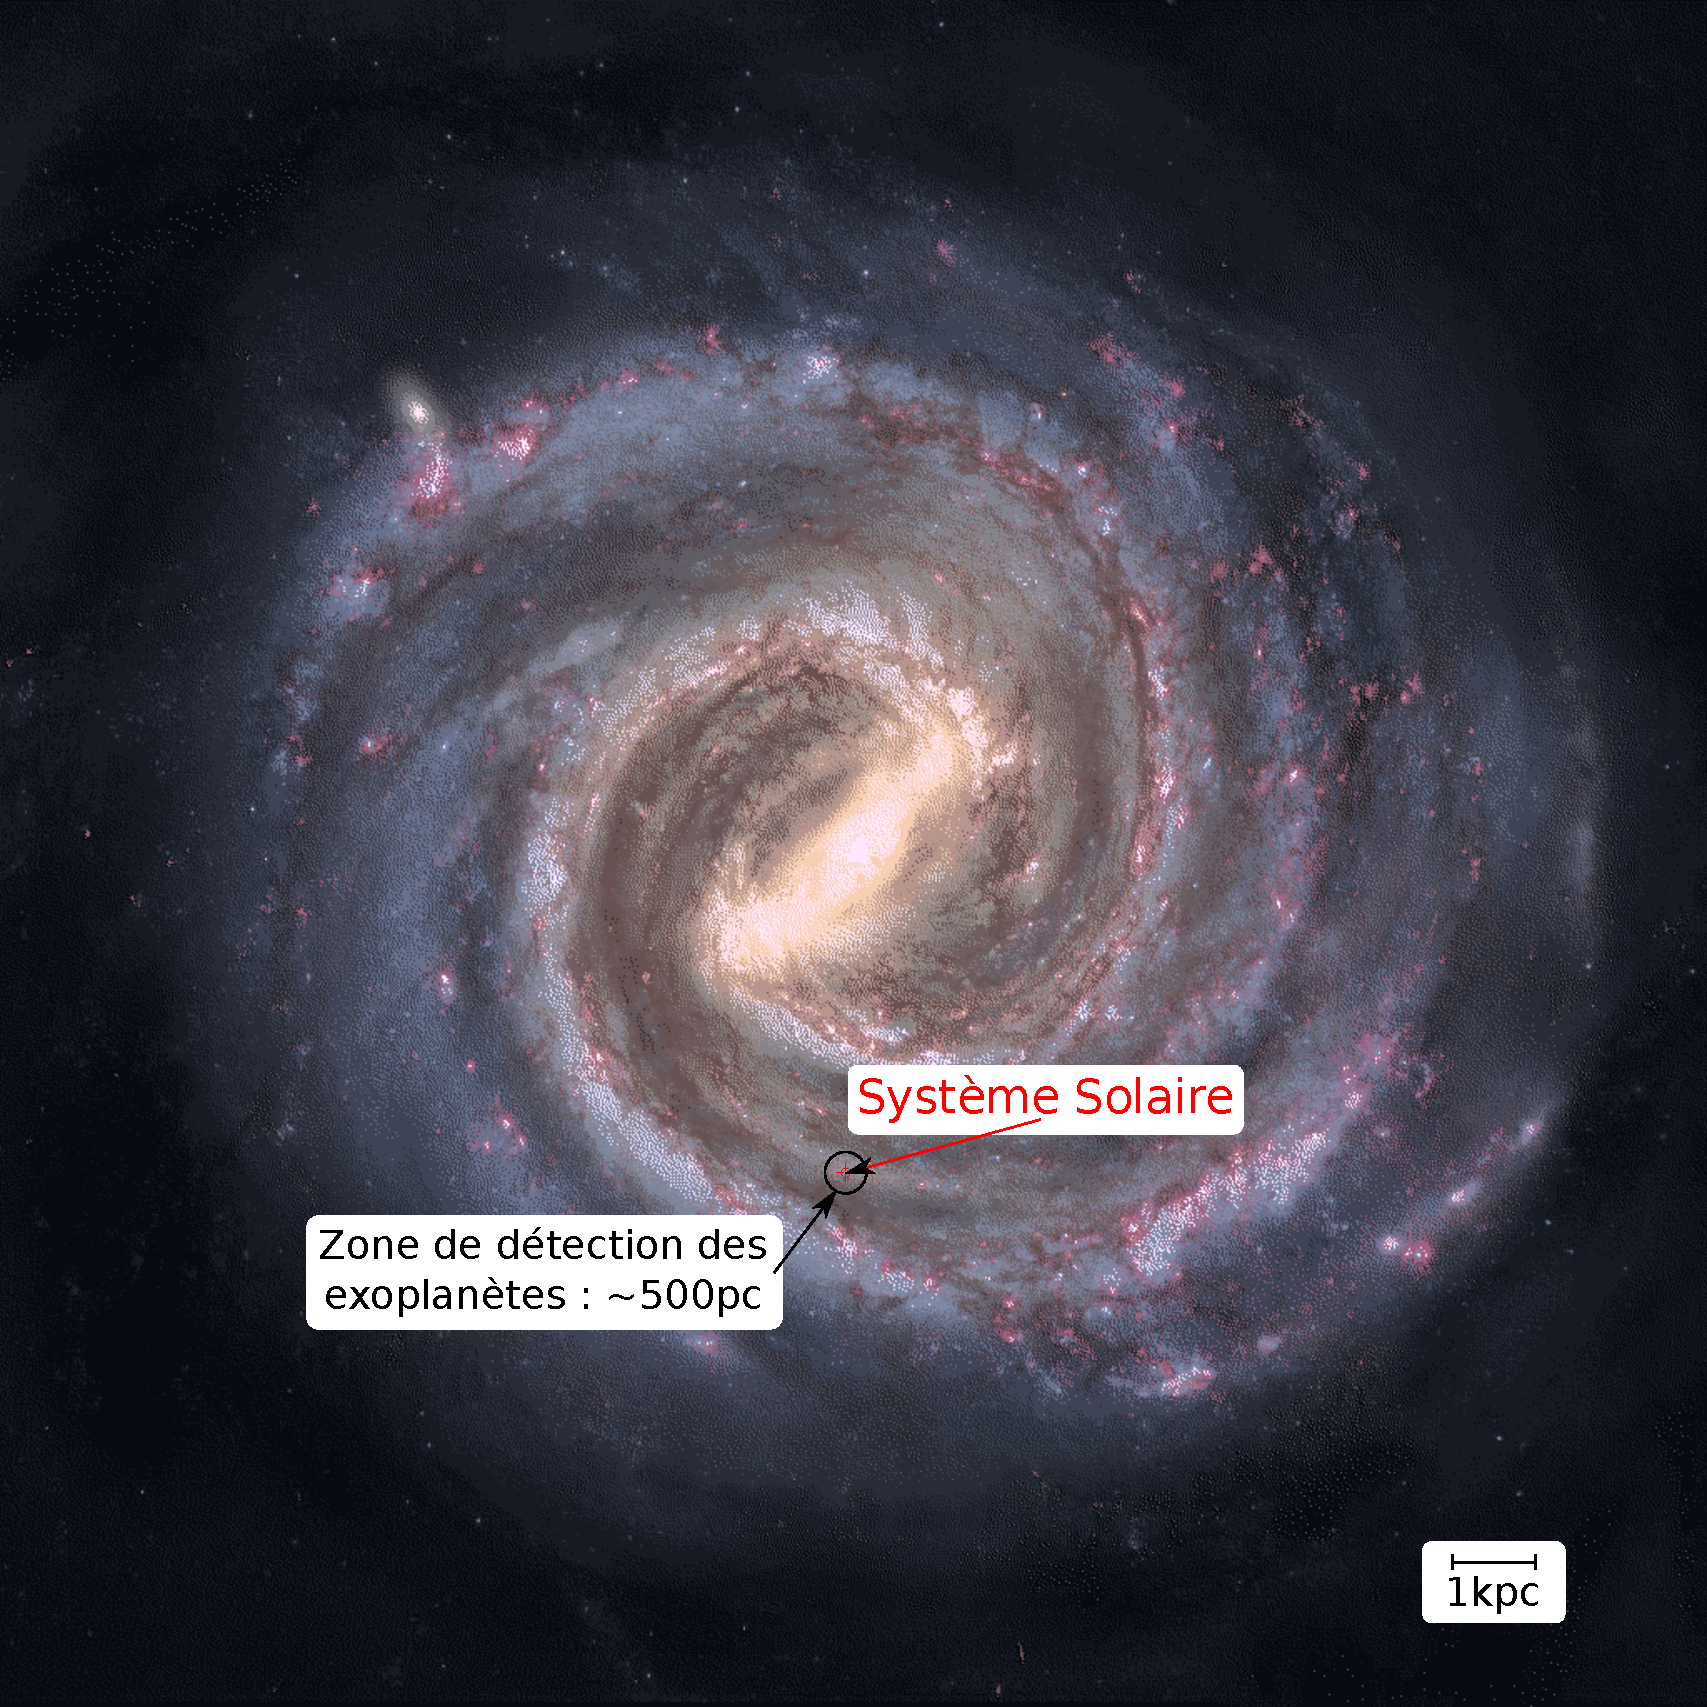
\includegraphics[width=0.45\linewidth]{figure/milky_way_exoplanets.pdf}
\caption{Image de la voie lactée avec indication de la position approximative du système solaire ainsi que de la zone (en noir) contenant la majorité des exoplanètes détectées à ce jour.}\label{fig:milky_way_exoplanet}
\end{figure}


En multipliant les méthodes de détections et les instruments, et surtout en ayant de plus en plus de planètes, il devient possible d'estimer la probabilité pour qu'une étoile héberge au moins une planète \citep{mayor2011road}. D'autres études estiment même la sensibilité de cette fréquence d'occurence en fonction de paramètres stellaires \citep{fischer2005planet, johnson2007new, howard2012occurrence} ou planétaires \citep{mayor2011road, howard2010occurrence}. 

Mais le point qui me semble le plus intéressant est la découverte de types de planètes qui n'existent pas dans le système solaire. En un mot : diversité. Que ce soient les jupiters chauds, comme \object{51 Peg b} ou les super terres comme \object{Gliese 1214 b}, ces planètes n'ont pas d'équivalent dans le système solaire. Ces variétés de composition, de taille, de systèmes nous offrent un champ de connaissance toujours plus grand dans lequel tester nos modèles de formations planétaire. Ils nous permettent aussi de mieux comprendre notre propre système et comment il s'est formé, et surtout de le placer dans cette immense horlogerie qu'est le catalogue de systèmes exoplanétaires à notre disposition.

%TODO HERE